\chapter{Preliminaries}
\label{sec:preliminaries}

%\section{Semantic Web}

%\section{RDF}
%Definition RDF Graph: Let there be pair-wise disjoint sets \ldots.

%\section{SPARQL}
%SPARQL is a recursive acronym for SPARQL protocol and RDF query language.
%Data query langague, Data modification language, Data definition language.

%\begin{figure}[htb]
%\centering
%Source: https://upload.wikimedia.org/wikipedia/commons/e/e4/Semantic_Web_Layer_Cake_Scheme.png?utm_source=commons.wikimedia.org&utm_campaign=index&utm_content=original
%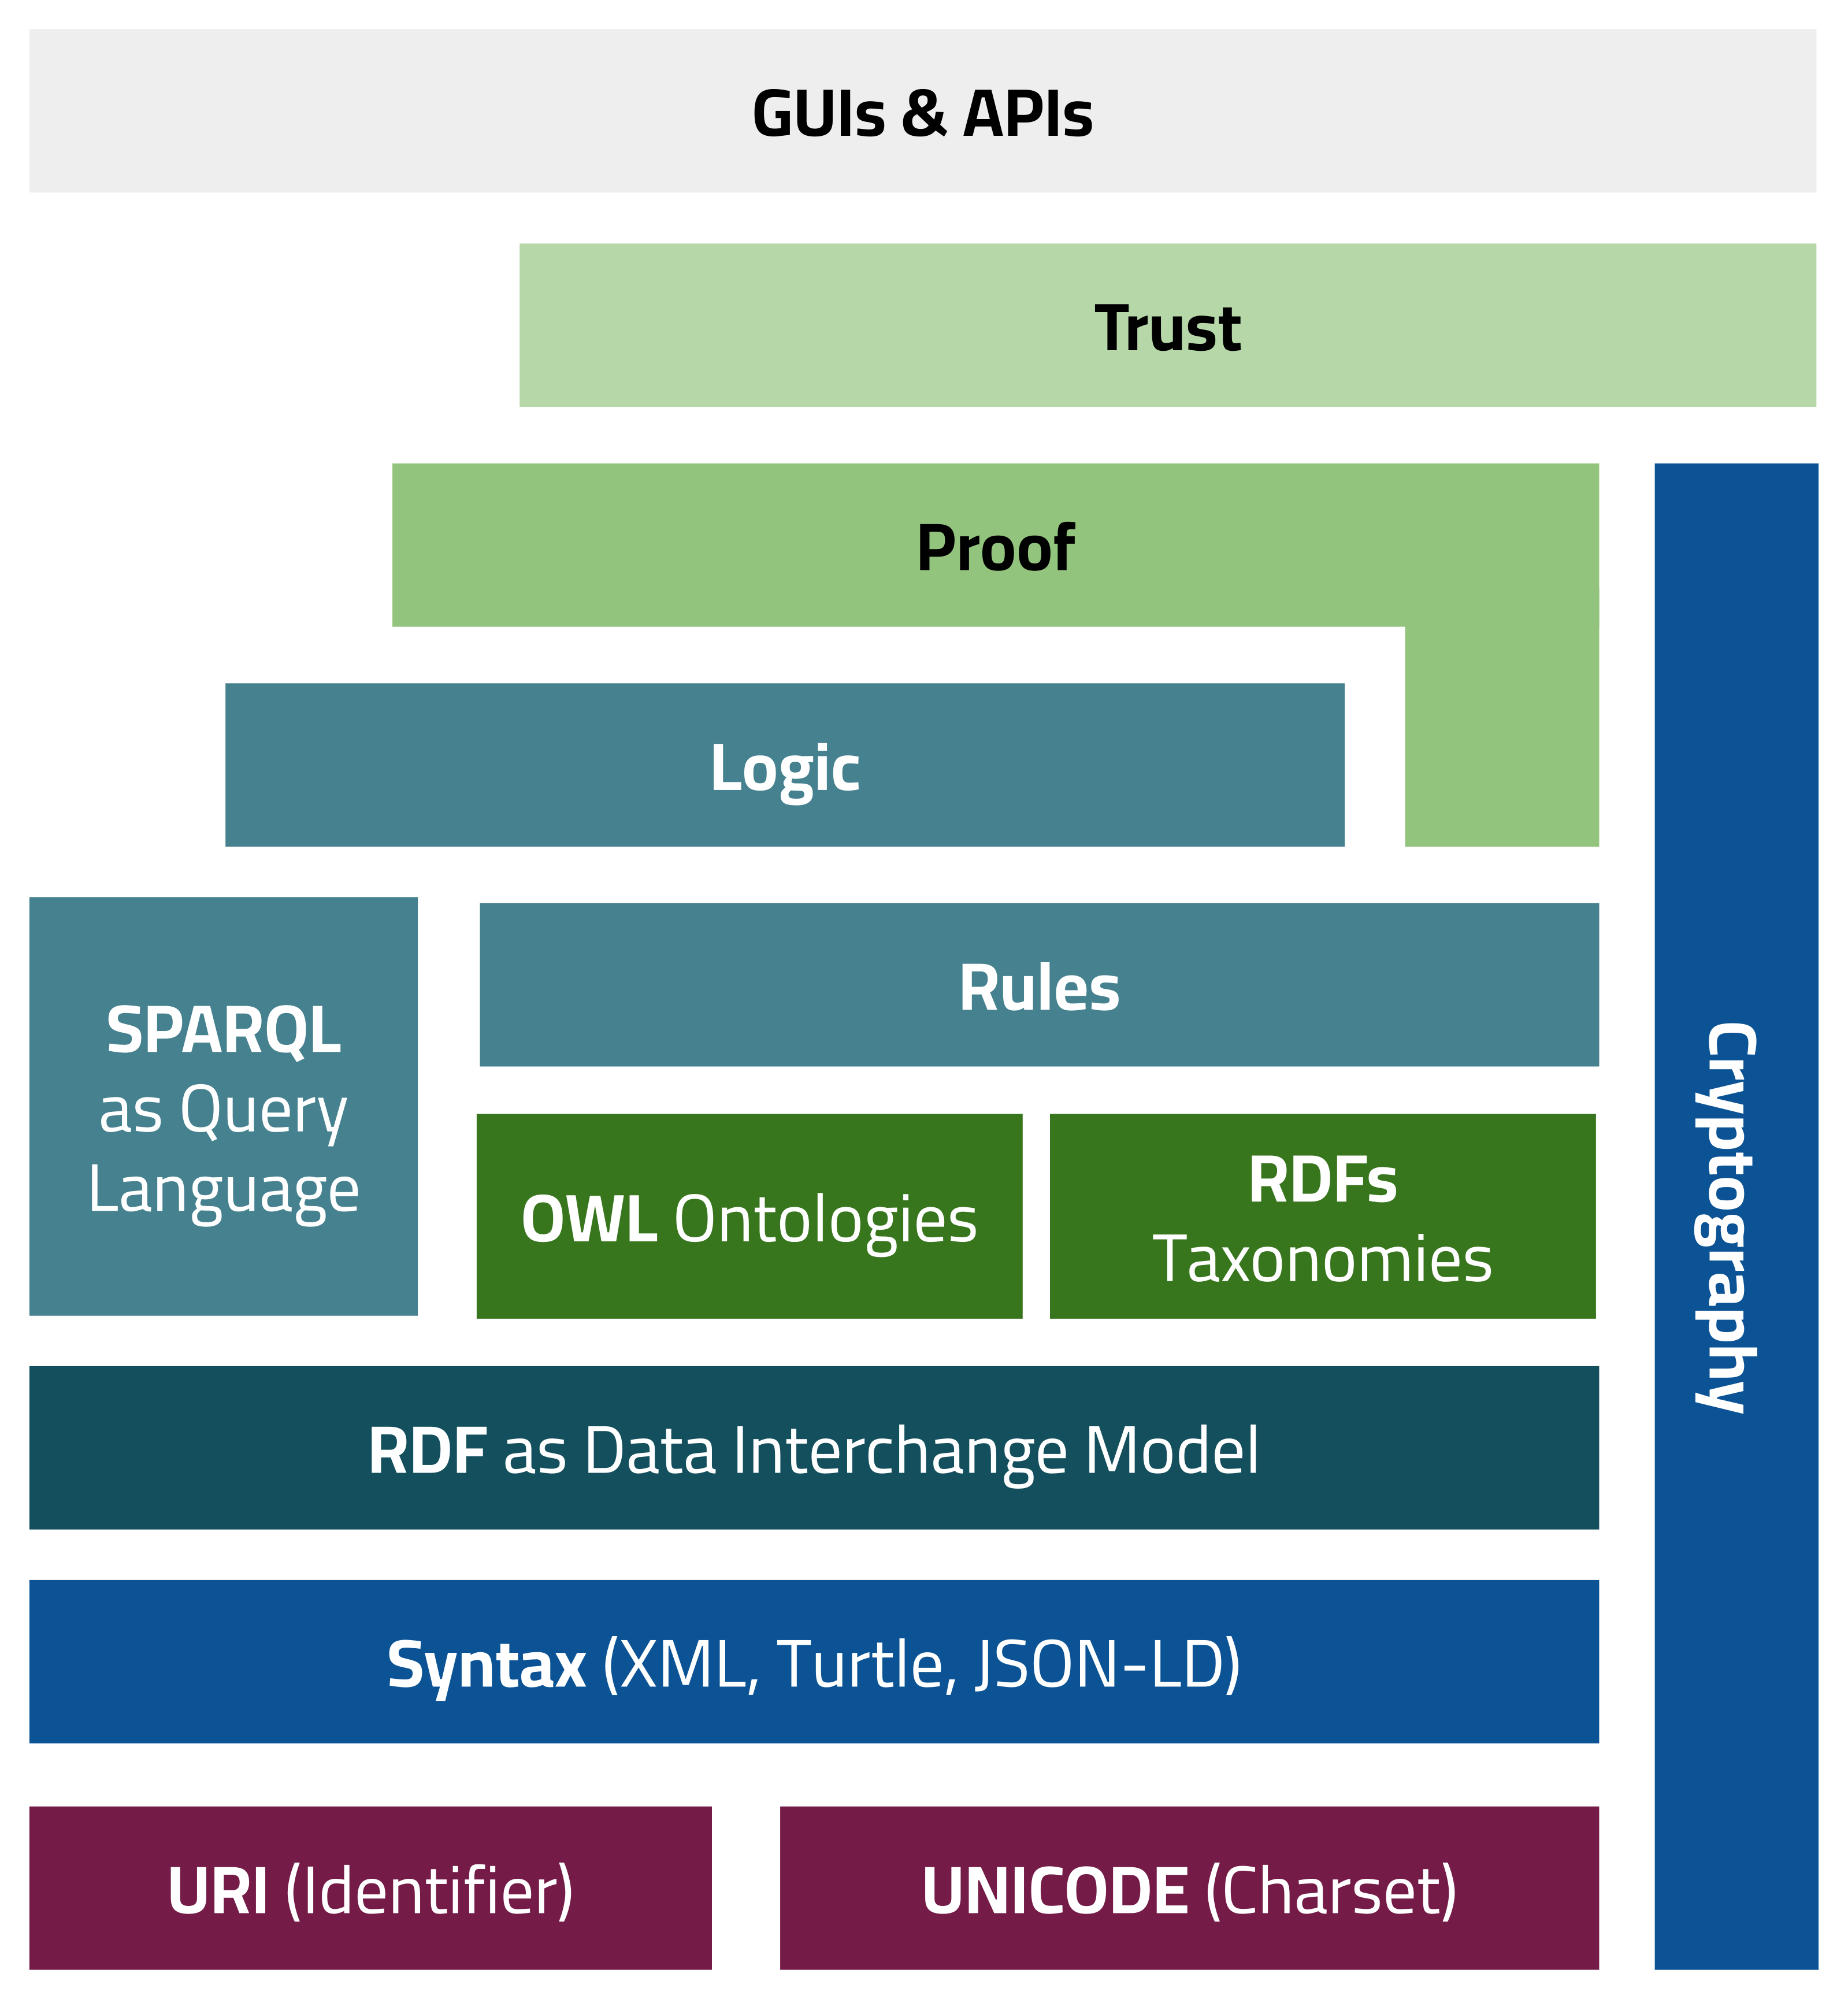
\includegraphics[width=\textwidth]{images/Semantic_Web_Layer_Cake_Scheme}
%\caption{Components of the Semantic Web Stack.}
%\caption*{\small{Source: \url{https://upload.wikimedia.org/wikipedia/commons/e/e4/Semantic_Web_Layer_Cake_Scheme.png}}}
%\label{fig:semantic-web-stack}
%\end{figure}

\section{The Semantic Web}
The vision of the Semantic Web, first described in \cite{sciam01}, is about
computer agents being able to understand the ``\emph{meaning}'' of some of
the content on the Web. By that we do not mean that agents magically become as
intelligent as humans, but rather that content is published in a form that
enables machines to easily gather information about things, and eventually
allows them to apply formal logic reasoning to that content.
Consider for example the query of finding
inexpensive hotels in the vicinity of a given location which offer certain
services such as cable TV and a swimming pool.
Traditional agents would have a hard time determining the answer to such task.
They would have to rely on data scraping or would require specialized code in
order to deal with the many non-standard APIs sites nowadays provide. Once they
manage to obtain the necessary data for answering the query, there is still the
problem of how to account for information that may become available in the future, such as what TV channels
are actually offered. But there is even another problem: Agents
supposedly solving the same problem, given the exact same query, and the exact same data to operate on, may come to different conclusions.
This happens due to the data lacking a defined
meaning.\footnote{Or agents not adhering to it. But that is beside the point.}
For example one agent may
interpret ``hotels'' as to include ``motels'' as well, while another agent may follow different semantics.
These are the basic problems addressed by the Semantic Web.
One of its fundamental properties is the implication of a
\emph{Web of Data} - a web made up of links between individual pieces of data
as opposed to the traditional links between documents\cite{WebOfData}.
The main reason is that data is a prerequisite for reasoning. Traditional
(e.g. HTML and XML) documents with their sheer endless amounts of different schemas
are unsuitable for uniform data access.

In order to realize the Semantic Web, an architecture of technologies has been
proposed, which is known as the \emph{Semantic Web Stack}.
It is depicted in Figure~\ref{fig:SemanticWebStack}.
In the following sections we will discuss the components which were
relevant to this thesis.

\begin{figure}[htb]
\begin{threeparttable}
\centering
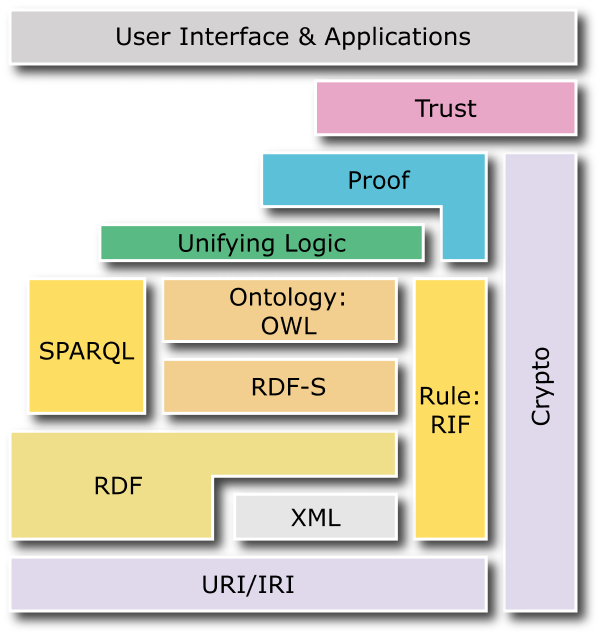
\includegraphics[width=0.6\textwidth]{images/SemanticWebStack/SemanticWebStack}
\begin{tablenotes}
\footnotesize
\item Source: \url{http://www.w3.org/2007/Talks/0130-sb-W3CTechSemWeb/#(24)}
\end{tablenotes}
\end{threeparttable}
\caption{Components of the \emph{Semantic Web Stack}}
\label{fig:SemanticWebStack}
\end{figure}



%\begin{figure}[tbh]
%\centering
%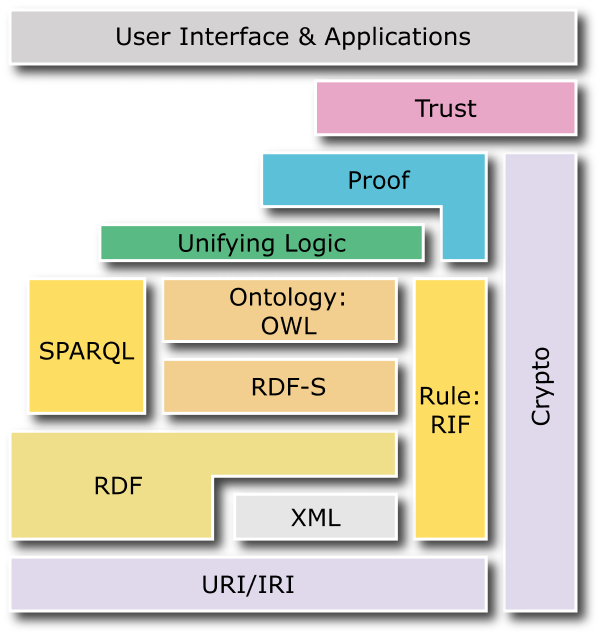
\includegraphics[width=8cm]{images/SemanticWebStack/SemanticWebStack}
%\caption{Components of the Semantic Web Stack}
%Source: \url{http://www.w3.org/2007/Talks/0130-sb-W3CTechSemWeb/#\%2824\%29}
%\label{SemanticWebStack}
%\end{figure}

\section{Uniform Resource Identifiers}
A Uniform Resource Identifier (URI) is a ``compact sequence of characters
that identifies an abstract or physical resource''\cite{URISpec}.
It is important to understand that the sole purpose of URIs is to
identify resources, but not to interact with them. As such they can be used to
identify \emph{anything} - so any concept one can think of, such as websites,
books, people or numbers. The dereferencable subset of URIs - that is the set
of URIs identifying machine accessible resources such as websites - is
known as Uniform Resource Locators (URLs). Identifying things
with URLs has the advantage that more information about the thing may be retrieved upon
dereferencing them. As a side note, a URL may both identify a thing and point
to a description of that thing, which makes its meaning ambiguous.
For example the URL \url{http://en.wikipedia.org/wiki/European_Union} could
refer to both the ``European Union'' as an organization and the article on Wikipedia.
Solutions to disambiguate the meanings are given in \cite{CoolURIs}.
For convenience URIs are often abbreviated using
\emph{namespace prefixes}. In regard to the example above, if
we somewhere stated that \texttt{enwiki} is an abbreviation of
\url{http://en.wikipedia.org/wiki/} we could have written
\url{enwiki:European_Union} instead.

\section{The Resource Description Framework}
The Resource Description Framework (RDF) is used to represent
information on the Web\cite{RDFConceptsAndAbstractSyntax}.
The framework defines two things: A \emph{data model} for
representing arbitrary statements about resources, and a basic \emph{vocabulary} which
can be used to give statements a defined meaning.
Since RDF is intended for the Web, it is natural that things are identified with
URIs. Furthermore RDF supports anonymous resources and literals such as strings
and integers.
A \emph{statement} consists of three parts namely
\emph{subject}, \emph{predicate} and \emph{object} where the set of
values they can take is shown below:
\begin{table}[!h]
\centering
\begin{tabular}{lccc}
\toprule
Part      &URI        &Anonymous  &Literal    \\
\midrule
Subject   &\checkmark &\checkmark             \\
Predicate &\checkmark                         \\
Object    &\checkmark &\checkmark &\checkmark \\
\bottomrule
\end{tabular}
\caption{Valid values within an RDF statement}
\end{table}



%\begin{table}
%\centering
%\begin{tabular}{|l|l|l|l|}
%\hline
%Part      & URI & Anonymous  & Literal \\
%Subject   &   x &          x &         \\
%Predicate &   x &            &         \\
%Object    &   x &          x &       x \\
%\hline
%\end{tabular}
%\caption{Valid values within a statement.}
%\end{table}

Since the object of one triple may appear as the subject in another
triple it is easy to see that a triple can be seen as an edge in a
directed labeled graph. Therefore a set of triples is also called a
\emph{graph}. Anonymous resources are usually referred to as
\emph{blank nodes}. \\
It is worth pointing out that literals may be either plain or typed. A plain
literal is a combination of a string with an optional language tag.
A typed literal is a combination of string and a URI denoting its data type. This
data type constrains the set of values that may be assigned to the string.

A couple of RDF statements is shown in Listing~\ref{lst:SimpleRDF}:
In this example this resource \texttt{ex:London} shall denote the city of
London. The first line states that its label in English is ``London''.
The second line states that the population is an integer of value {8278251}.

%\begin{lstlisting}[label=lst:SimpleRDF, caption=Examples of RDF statements,captionpos=b,style=rdf]
%ex:London ex:label "London"@en .
%ex:London ex:population 8278251^^xsd:integer
%\end{lstlisting}

\begin{listing}[H]
\caption{Examples of RDF statements}
\label{lst:SimpleRDF}
\begin{minted}{turtle}
ex:London ex:label "London"@en .
ex:London ex:population 8278251^^xsd:integer
\end{minted}
\end{listing}

%\begin{figure}
%\centering
%\begin{minipage}[t]{0.8\textwidth}
%\end{minipage}
%\caption{Examples of RDFstatements}
%\end{figure}


\subsection{Syntaxes}
The RDF data model itself is an abstract syntax which means that it is
independent of any particular representation or encoding.
Several concrete syntaxes exist which vary in readability, expressiveness and
tool support.

\subsubsection{RDF/XML} is an XML based syntax and therefore has the same
advantages and disadvantages as basically any other XML based syntax: On the one hand there
exists a wide range of tools which make parsing and processing of such data
relatively easy for machines. On the other hand XML documents contain a lot of
syntactic noise which makes human reading and writing of actual data
harder than it ought to be. However, RDF/XML is a
mandatory exchange syntax\cite{OWL2DocumentOverview} for some RDF-based
languages, such as
\mbox{OWL 2}\footnote{Discussed in \ref{RDFBasedLanguages}}.
This means that the syntax must be supported by tools dealing with that
language.

\subsubsection{N-Triples, Turtle and {Notation3}} are plain text based concrete
syntaxes which are more human-friendly as the XML variant. N-Triples is a subset of Turtle and Turtle is a subset of
\mbox{Notation3} which means that they are not completely different syntaxes
but merely syntaxes with varying degrees of expressivity, as shown in
Figure~\ref{RDFSyntaxesVennDiagramm}.

\begin{figure}[htb]
\begin{threeparttable}
\centering
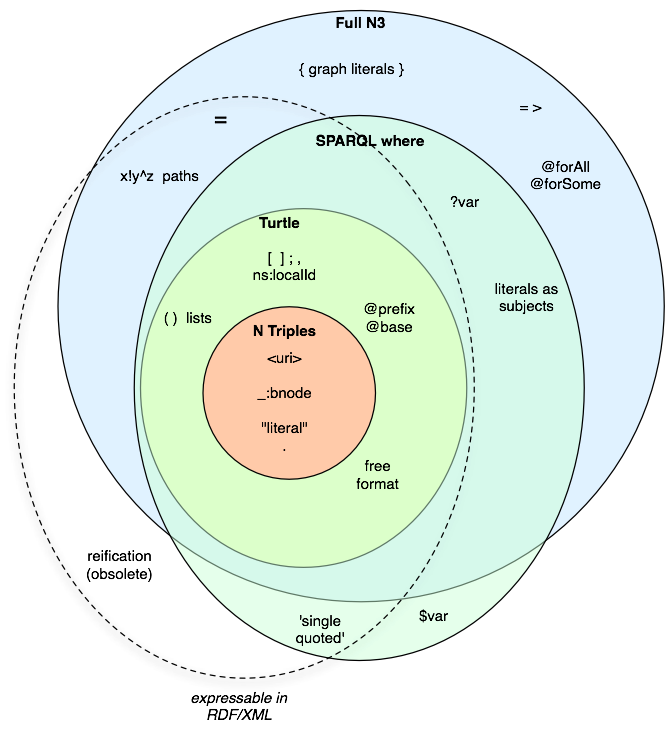
\includegraphics[width=0.8\textwidth]{images/RDFSyntaxesVennDiagramm}
\begin{tablenotes}
\footnotesize
\item Source: \url{http://www.w3.org/DesignIssues/Notation3}
\end{tablenotes}
\end{threeparttable}
\caption{Set relations between the various syntaxes}
\label{RDFSyntaxesVennDiagramm}
\end{figure}



Besides the syntaxes listed here, others came into existence like
TriX, TriplesML, or Regular XML RDF (RXR). However none of them seems to play an
important role.


\section{SPARQL and SPARUL}
\emph{SPARQL}\cite{SPARQLSpec} is a recursive acronym for ``SPARQL Protocol
and RDF Query Language''. It is the query language for the Semantic Web and is therefore a language adapted to
the RDF data model. Since RDF data forms a graph, the central part of the SPARQL
query language are graph patterns. These graph patterns look similar to graphs
written in Turtle with the exception that variables may appear anywhere as a
subject, predicate, or object. Another important part of a SPARQL query is the
\emph{query form} which controls the result being returned based on the
data matched by the graph pattern of the query. Four query forms are given,
namely SELECT, CONSTRUCT, DESCRIBE and ASK. The first two return the result as
a table and a graph, respectively. DESCRIBE is used to fetch data about
individual resources, and ASK serves to determine whether a query yields any
result at all.

\emph{SPARUL}\cite{SPARQLUpdate} is the corresponding data manipulation
language also known as \emph{SPARQL/Update}. It introduces the INSERT, DELETE
and the more general MODIFY statement. The latter is a combination of the
first two. In essence it works like a
SPARQL CONSTRUCT query that inserts and/or removes the result set from the
store. Table~\ref{tab:SPARQLExample} shows some example queries.


%\begin{table}[!h]
%\centering
%\begin{tabular}{lll}
%\toprule
%Select      & Construct & Insert  \\
%\midrule
%\begin{minipage}{2.9cm}
%\begin{lstlisting}[style=sparql, escapechar=\%]
%SELECT ?name
%FROM <http://ex.org> {
%  ?p ex:type ex:Person .
%  ?p ex:name ?name .
%}
%%%
%\end{lstlisting}
%\end{minipage}
%&
%\begin{minipage}{2.8cm}
%\begin{lstlisting}[style=sparql]
%CONSTRUCT {
%  ?s rdfs:label ?o .
%}
%FROM <http://ex.org> {
%  ?s ex:name ?o .
%}
%\end{lstlisting}
%\end{minipage}
%&
%\begin{minipage}{3.5cm}
%\begin{lstlisting}[style=sparql, escapechar=\%]
%INSERT DATA
%INTO <http://ex.org> {
%  ex:Anne ex:knows ex:Bob .
%}
%
%%%
%\end{lstlisting}
%\end{minipage}
%\\
%\bottomrule
%\end{tabular}
%\caption{Examples of simple SPARQL queries}
%\label{tab:SPARQLExample}
%\end{table}

\begin{table}[!h]
\centering
\begin{adjustbox}{width=\textwidth,center}  % ← scales entire table to text width
\begin{tabular}{ccc}
\toprule
\textbf{SELECT} & \textbf{CONSTRUCT} & \textbf{INSERT} \\
\midrule

% --- SELECT block ---
\begin{minipage}{0.3\linewidth}
\begin{minted}[fontsize=\scriptsize,autogobble,frame=none,bgcolor=lightblue]{sparql}
SELECT ?name
FROM <http://ex.org> {
  ?p ex:type ex:Person .
  ?p ex:name ?name .
}
\end{minted}
\end{minipage}
&
% --- CONSTRUCT block ---
\begin{minipage}{0.3\linewidth}
\begin{minted}[fontsize=\scriptsize,autogobble,frame=none,bgcolor=lightblue]{sparql}
CONSTRUCT {
  ?s rdfs:label ?o .
}
FROM <http://ex.org> {
  ?s ex:name ?o .
}
\end{minted}
\end{minipage}
&
% --- INSERT block ---
\begin{minipage}{0.35\linewidth}
\begin{minted}[fontsize=\scriptsize,autogobble,frame=none,bgcolor=lightblue]{sparql}
INSERT DATA
INTO <http://ex.org> {
  ex:Anne ex:knows ex:Bob .
}
\end{minted}
\end{minipage}
\\
\bottomrule
\end{tabular}
\end{adjustbox}
\caption{Examples of simple SPARQL queries}
\label{tab:SPARQLExample}
\end{table}

\section{Triple Stores and Query Engines}
Triple stores are database systems capable of storing and retrieving RDF data.
Some implementations are based on relational database technology which means
that they internally rewrite SPARQL and SPARUL queries to SQL
statements. There also exist native implementations of triple stores such as
\emph{Sesame}\footnote{\url{http://www.aduna-software.com/technology/sesame}},
\emph{Virtuoso}\footnote{\url{http://virtuoso.openlinksw.com/}} and
\emph{AllegroGraph}\footnote{\url{http://www.franz.com/agraph/allegrograph/}}.
Engines like
\emph{Triplify}\footnote{\url{http://triplify.org}}
and \emph{D2R}\footnote{\url{http://www4.wiwiss.fu-berlin.de/bizer/d2r-server/}}
allow the definition of mappings from legacy relational data to RDF. The latter
engine even supports querying with SPARQL. The Berlin
Benchmark\cite{BerlinSparql} compared the performance of native and
rewriting-based triple stores. At that time rewriters outperformed native stores
with increasing dataset size.


\section{Ontologies and Ontology Languages}
``An ontology is a formal, explicit specification of a shared
conceptualization. Conceptualization refers to an abstract model
of some phenomenon. Explicit means that the types of concepts
used, and the constraints on their use are explicitly defined.
Formal refers to the fact that the ontology should be machine-
readable. Shared reflects the notion that an ontology captures
consensual knowledge, that is, it is not private of some
individual, but accepted by a group.''\cite{OntologyDefinition}
Ontologies are represented using \emph{ontology languages}.
Many of such languages exist which vary greatly in
expressivity, computational complexity and decidability. Some of them are
presented in the following section.

\subsection{RDFS, OWL and OWL 2}
\label{RDFBasedLanguages}
RDF schema (RDFS), the Web Ontology Language
(OWL\footnote{This is not a typo: \scriptsize\url{http://lists.w3.org/Archives/Public/www-webont-wg/2001Dec/0169.html}}),
and its successor \mbox{OWL 2} are ontology languages which have gained significant importance in the context of the Semantic Web.
OWL and \mbox{OWL 2} can be broken down into sub languages which trade
expressive power for efficiency of reasoning.
OWL's sublanguages are OWL Lite, OWL DL and OWL Full.
The sublanguages of \mbox{OWL 2}, better known as \emph{profiles}, are
\mbox{OWL 2 EL}, \mbox{OWL 2 QL} and \mbox{OWL 2 RL}. A major difference between
the two versions of OWL is, that the profiles were designed to be especially
suitable for certain types of applications.

These languages have the following basic concepts in common:
\begin{itemize}
  \item \emph{Individuals} are primitive entities. As such they are no sets
  which distinguishes them from classes.
  \item \emph {Classes} are sets of individuals. The members of a class are
  called \emph{instances}. An individual may belong to multiple classes which
  are referred to as its \emph{types}.
  \item \emph {Literals} are data values such as strings or integers.
  \item \emph {Properties} are relations between individuals, classes
  and literals.
\end{itemize}
Although the aforementioned languages are all based on these concepts, their
expressivity varies. For example while it is  legal in RDFS to model classes of
classes, this is considered illegal in \mbox{OWL DL}.

Ontologies form the backbone of the Semantic Web as they enable us to give
meanings to resources.
For example, assume we are given the following statements:
%\begin{figure}[!h]
%\begin{small}
%\begin{lstlisting}[language=turtle]
%Leipzig a City.
%Leipzig locatedIn Saxony.
%Saxony locatedIn Germany.
%\end{lstlisting}
%\end{small}
%\end{figure}

\begin{listing}[!h]
\centering
\begin{minted}[fontsize=\footnotesize,autogobble,frame=none,bgcolor=lightblue]{turtle}
:Leipzig a :City .
:Leipzig :locatedIn :Saxony .
:Saxony :locatedIn :Germany .
\end{minted}
\caption{Simple RDF graph in Turtle syntax}
\label{fig:turtle-example}
\end{listing}

If a machine wanted to find all German cities based on these
statements, it would have to infer the fact \texttt{Leipzig locatedIn Germany}. Although a
special treatment of the \texttt{locatedIn} property could be hard coded into an
application, the point of ontologies is that this treatment can be explicitly
stated: In our example we would have to add the triple
\texttt{locatedIn a owl:TransitiveProperty} in order to define
\texttt{locatedIn} as a transitive property. As a consequence, any application
understanding the ontology language is then able to draw the correct
conclusions.


\subsection{Manchester OWL Syntax (MOS)}
\label{sec:MOS}
This syntax's main goal is to simplify the reading and writing of class
expressions\footnote{Also known as class descriptions.},
especially for people who do not have Description Logic (DL)
background\cite{ManchesterOWLSyntax}. It achieves that goal by
hiding the formal symbols typically used in this field behind English
keywords and introducing a grammar where these keywords appear in locations
that make them look more natural. An example is shown in
Figure~\ref{fig:MOSExample}.

\begin{figure}[!h]
\centering
\begin{tabular}{ll}
\begin{minipage}[t]{0.4\textwidth}
\begin{scriptsize}
\begin{math}
\texttt{Pizza} \sqcap (\\
\neg (\exists \texttt{hasTopping}.\texttt{MeatTopping}) \sqcup \\
\neg (\exists \texttt{hasTopping}.\texttt{FishTopping}) )
\end{math}
\end{scriptsize}
\end{minipage}
&
\begin{minipage}[t]{0.4\textwidth}
\begin{scriptsize}
\begin{verbatim}
Pizza THAT
NOT hasTopping SOME
(MeatTopping OR FishTopping)
\end{verbatim}
\end{scriptsize}
\end{minipage}
\end{tabular}
\caption{DL Syntax vs MOS syntax}
\label{fig:MOSExample}
Definition of the class ``Vegetarian Pizza'' as a Pizza without Meat
and Fish toppings in traditional DL syntax (left) and MOS syntax (right)
\end{figure}

\subsubsection{Reification and Annotations}
Reification, sometimes called ``nounification'' or ``thingification'', refers
to making a statement about a statement. If we want to represent the
statement ``Anne knows Bob claims Charlie'' in RDF we first have to introduce a
new resource - usually a blank node - which represents the base statement
``Anne knows Bob''. Once such a resource exists, it can be used in further
statements. RDF provides a reification vocabulary. However it was
declared deprecated because of unclear semantics.
Eventually \emph{annotations} were introduced in \mbox{OWL 2}.
Instead of making statements about statements, the view point has changed to
annotating statements. Annotations are logically irrelevant, which means that
they do not affect the truth value of the statement being annotated, and are
therefore ignored by a reasoner. An example of the RDF-reification and OWL 2
annotation approaches is given in Table~\ref{tab:ReificationVsAnntations}.

\begin{table}[!h]
\centering
\begin{tabular}{ll}
\toprule
RDF-Reification & OWL 2 Axiom Annotations \\
\midrule
\begin{minipage}{5cm}
\begin{lstlisting}[language=turtle]
_:b a rdf:Statement
_:b rdf:subject :s
_:b rdf:predicate :p
_:b rdf:object :o
\end{lstlisting}
\end{minipage}
&
\begin{minipage}{5cm}
\begin{lstlisting}[language=turtle]
_:b a owl:Axiom
_:b owl:annotatedSource :s
_:b rdf:annotatedProperty :p
_:b rdf:annotatedTarget :o
\end{lstlisting}
\end{minipage}
\\
\bottomrule
\end{tabular}
\caption{RDF-Reification vs OWL 2 Axiom Annotations}
\label{tab:ReificationVsAnntations}
\end{table}


\section{Linked Data}
The fundamental feature which contributed to the success of the World Wide Web
was the hyperlink. In fact without links, there would not be any web at all.
However most links are untyped relations between documents (e.g. HTML or XHTML).
While this is of no problem for humans, it greatly complicates the tasks for
machine agents to explore and find relevant information. On
the one hand an agent has to deal with the various schemas of these documents
and on the other hand it must somehow decide which links to follow.
In contrast, Linked Data is about making typed links between pieces of
(RDF) data.
This makes it easier for machine agents to follow links and
retrieve data that seems interesting to them just like humans.
Note that already existing technologies for
naming resources (URIs), resolving these names to physical addresses (DNS),
and transferring data from them (HTTP)
can be reused directly. The following principles for publishing Linked Data
are adapted from \cite{LinkedDataDesignIssues} and are summarized as:
\begin{itemize}
\item Name things using
HTTP\footnote{As HTTP is widely supported.}
URIs\footnote{As any URI may already be or eventually become a URL, making it
machine accessible.}. Even better, use URLs.
\item Upon dereferencing such URL, return an RDF dataset describing that
resource. Additionally that dataset should\ldots
\item \ldots contain URLs that can be further resolved to more RDF data.
\end{itemize}

\subsubsection{Content negotiation} is a feature of HTTP which enables user agents
to choose from different representations for a given resource identified by a
URI. A browser could for example attempt to request websites in preferred languages
or images in preferred formats. Of course the server must support the requested
representation. By using content negotiation, it is possible that for the same
URI a browser would obtain a human readable HTML representation while another agent
would receive an RDF representation.

\subsubsection{The Linked Open Data cloud} (LOD cloud), depicted in
Figure~\ref{fig:LODCloud}, is the result of the
\emph{Linking Open Data} W3C Community
project\cite{LODProject}: Within this project various
open datasets are (converted to and) published as RDF and interlinked with
each other. As a consequence, information about entities residing in
multiple, partly even heterogeneous datasets can be accessed in a uniform way.

Notably, DBpedia plays the role of a \emph{linking hub} within the LOD cloud.
The main reasons that led to this development are:
\begin{enumerate}
  \item The meaning of (most) EnWiki article names does not change
  (significantly) over time as shown in \cite{HarvestingWikiConsensus}, making
  them suitable for knowledge representation.
  The same is valid for DBpedia URIs as they are based on these names.
  \item EnWiki covers multiple domains such as movies, places,
  organizations. The corresponding identifiers are
  attractive for reuse in these domains due to their stable meaning.
  As in the previous point, DBpedia benefits directly from EnWiki.
  \item In contrast to Wikipedia, DBpedia URIs can be resolved to RDF via the
  Linked Data interface. As DBpedia itself contains links to various
  other knowledge bases, linking to DBpedia indirectly interlinks with them.
\end{enumerate}
\begin{figure}[htb]
\begin{threeparttable}
\centering
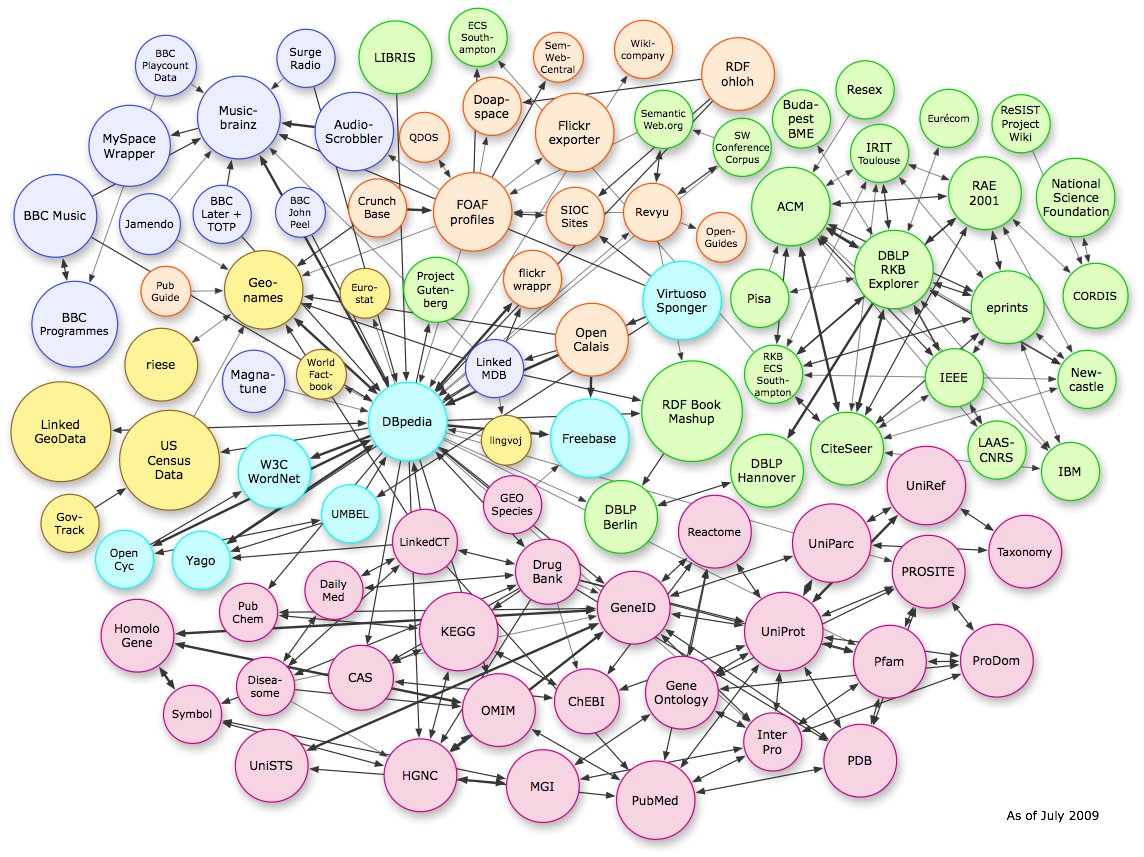
\includegraphics[width=\textwidth]{images/lod-datasets_2009-07-14_colored}
\begin{tablenotes}
\scriptsize
\item Source: \url{http://www4.wiwiss.fu-berlin.de/bizer/pub/lod-datasets_2009-07-14_colored.png}
%\item [~] Source: \url{http://www4.wiwiss.fu-berlin.de/bizer/pub/lod-datasets_2009-07-14_colored.png}
\end{tablenotes}
\end{threeparttable}
\caption{The \emph{Linked Open Data cloud}}
\label{fig:LODCloud}
\end{figure}

